\section{Wprowadzenie}
\label{sec:Wprowadzenie}

% TODO
Termin ,,Big Data'' odnosi się do wielkich zbiorów danych, często liczących nawet petabajty danych. Takie ilości danych powstają np. w wyniku obserwacji teleskopem. Tak ogromnych zbiorów danych nie da się już analizować konwencjonalnymi metodami -- tradycyjne, relacyjne bazy danych nie radziły sobie z przechowywaniem i analizą aż tak wielu informacji. Na dodatek dane te często bywają pozbawione wyraźnej struktury (np. posty na Twitterze), co jeszcze bardziej pogarszało performance takich baz danych.

Obecnie do analizy tak dużych ilości danych uzywa się platform takich jak Hadoop \cite{apache:hadoop}, czy platformy Google. Są to platformy rozproszone, oparte na specjalnie zaprojektowanych systemach plików (np. HDFS -- Hadoop Distributed File System, opisany w \cite{shvachko10}), na których stoją bazy danych NoSQL (HBase, BigTable). Do przetwarzania danych powstał paradygmat MapReduce \cite{dean08}, który w prosty sposób przeprowadza rozproszone obliczenia na danych przechowywanych w systemie. Aby ułatwić korzystanie z tych systemów powstały takie nakładki jak Apache Pig, które umożliwiają wykonywanie zapytań i obliczeń za pomocą prostych języków, nieco przypominających SQL.

Termin ,,Big Data'' staje się coraz popularniejszy. Wzrost zainteresowania tym tematem pokazuje poniższy wykres, na którym przedstawiono porównanie liczby zapytań w wyszukiwarce Google terminów ,,Big Data'' (kolor niebieski) oraz popularnego 2 lata temu ,,Cloud Computing'' \ref{fig:big_data_popularnosc} (kolor czerwony).

\begin{figure}[h]
\centerline{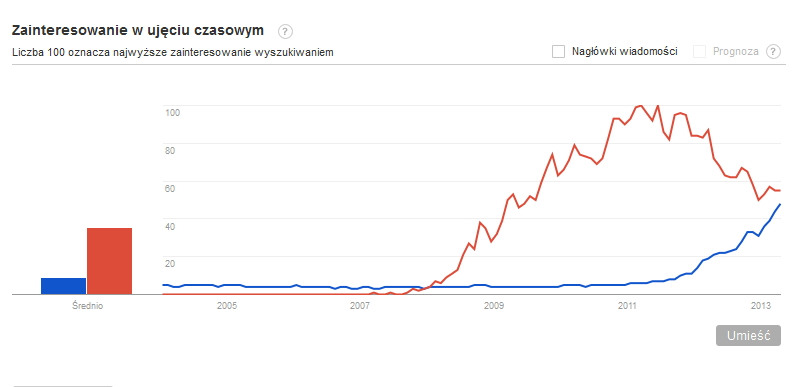
\includegraphics[scale=2.5]{obrazki/trend-big-data_cloud-computing.png}}
\caption{Porównanie popularności wyszukiwania terminów ,,Big Data'' (niebieski) oraz Cloud Computing (czerwony)}
\label{fig:big_data_popularnosc}
\end{figure}

Jak widać na wykresie zwłaszcza w przeciągu ostatniego roku zainteresowanie tematem Big Data gwałtownie zaczyna rosnąć.

% section wprowadzenie (end)
